%%%%%%%%%%%%%%%%%%%%%%%%%%%%%%%%%%%%%%%%%%%%%%%%%%%%%%
\section{はじめに}

 地震等に伴う電離圏の変動を観測するため,HF帯電波を用いたHFD観測という手法が取られている.このHFD(短波ドップラー)観測のデータは電離圏研究のためにオープンデータとして公開されており,自由な使用が認められている.\cite{hfd_report}\\
 現状,データ活用を促進するために数件の web アプリケーションが開発されている.しかし,設計時点で複数の言語が使用されている,ページの読み込みに時間がかかるなど,その多くが開発運用の困難性やユーザーエクスペリエンス等の観点で問題を抱えている.また,webアプリケーションの主な使用者となる電離圏の研究者から,いくつかの要望が出されている.それらをいくつか抜粋して,以下表1に示す.\\
\begin{table}[h]
  \centering
  \caption{webアプリケーションに対する要望の抜粋}
  \label{tab:requst}
  \begin{tabular}{l}
  \toprule
     ・周波数固定で全ての局を見せる\\
    ・局固定で全ての周波数を見せる\\
    ・局,周波数を選んでカスタムプロットしたい\\
    ・ダイナミックスペクトルを見たい\\
    ・PDF などの形に出力できると良い\\
    ・パンとズームができると良い
  \end{tabular}
\end{table}\\
 既存のwebアプリケーションにおける課題点の解消,及び研究者からの要望を反映したwebアプリケーションを提供するため,webアプリケーションの新規設計を行う.既存のwebアプリケーションにおける課題点を解消するため,ページレンダリング手法を考慮して開発を進めていく.本研究ではNext.jsと呼ばれるJavaScriptのフレームワークを用いて実装を行う.JavaScriptのUIライブラリの一つであるReact.jsがベースとなっており,サーバ機能も有しているため効率的なweb開発が可能である.また,サーバーサイドレンダリング(SSR)や静的サイト生成(SSG)といった機能を持つwebサイトの作成を得意とする.そのため,今回開発するwebアプリケーションの要件に合致していると判断した.\cite{next}\\
 本研究ではこのwebアプリケーションにおける web スクレイピングを用いてオープンデータが公開されているwebサイトからデータを取得する処理,および,取得したデータを整形してフロントエンドで扱いやすく整形する処理に焦点を当てる.また,使用する言語をwebアプリケーション開発全体で統一して管理コストの低減を図るため,webスクレイピングに関する処理はTypeScriptを用いて行う.\\
%%%%%%%%%%%%%%%%%%%%%%%%%%%%%%%%%%%%%%%%%%%%%%%%%%%%%%
\section{Webスクレイピングについて}

 webスクレイピングとは,web サイトから情報を抽出するコンピュータソフトウェア技術のことを指す.HTML フォーマットからテキストを抽出してスプレッドシートや json ファイル等の構造化データへの変換を行うことができ,web 上にあるデータを取得して扱うことを目的とする.web スクレイピングの手法としては,正規表現や DOM 解析,HTML パーサ等を用いたものがある.本研究では,ISRを用いたwebアプリケーションを設計するため,スクレイピングの処理に速度を求める必要がない.そのため,本研究では軽量でサーバへの負担が小さいcheerioをHTMLパーサとして用いる.
%%%%%%%%%%%%%%%%%%%%%%%%%%%%%%%%%%%%%%%%%%%%%%%%%%%%%%
\section{使用ライブラリ}
 本研究で使用した主なTypeScritpライブラリについて以下に示す.
%%%%%%%%%%%%%%%%%%%%%%%%%%%%%%%%%%%%%%%%%%%%%%%%%%%%%%
\subsection{Superagent}

 HTMLリクエストを送信することのできるモジュール.本研究ではHFD観測データが公開されているwebページからHTMLレスポンスとしてテキストデータを取得する際に用いる.\cite{superagent}
%%%%%%%%%%%%%%%%%%%%%%%%%%%%%%%%%%%%%%%%%%%%%%%%%%%%%%
\subsection{Cheerio}

 HTMLパーサにjQueryのサブセットを実装したもの.jQueryの関数を用いてスクレイピングの処理を行うことができる.本研究ではHTMLレスポンスからテキストデータだけを抜き出す際に用いる.\cite{cheerio}
%%%%%%%%%%%%%%%%%%%%%%%%%%%%%%%%%%%%%%%%%%%%%%%%%%%%%%
\section{実装}
%%%%%%%%%%%%%%%%%%%%%%%%%%%%%%%%%%%%%%%%%%%%%%%%%%%%%%
\subsection{目標}
 本開発では,Next.jsを用いて開発運用及びユーザーエクスペリエンスの観点で従来のものよりも優れたWebアプリケーションを作成することを目標とする.その中でも,本研究ではスクレイピングを用いてデータを取得し,それをフロントエンドで扱いやすいように整形する処理を行うことまでを目標とする.
%%%%%%%%%%%%%%%%%%%%%%%%%%%%%%%%%%%%%%%%%%%%%%%%%%%%%%
\subsection{スクレイピング処理}
 Superagentを用いて,HFドップラーのデータが公開されているwebサイト\cite{hfd}にHTMLリクエストを送る.返ってきたHTMLレスポンスからcheerioを用いてbodyを抜き出し,テキストデータに変換する.
%%%%%%%%%%%%%%%%%%%%%%%%%%%%%%%%%%%%%%%%%%%%%%%%%%%%%%
\subsection{データ整形処理}
 前項で取得したテキストデータはそのままでは扱いにくいため,扱いやすい形に整形する.例として,2020/11/20Sarobetsuのデータを示す.
 \begin{figure}[h]
   \centering
   \caption{Caption}
   \label{fig:my_label}
   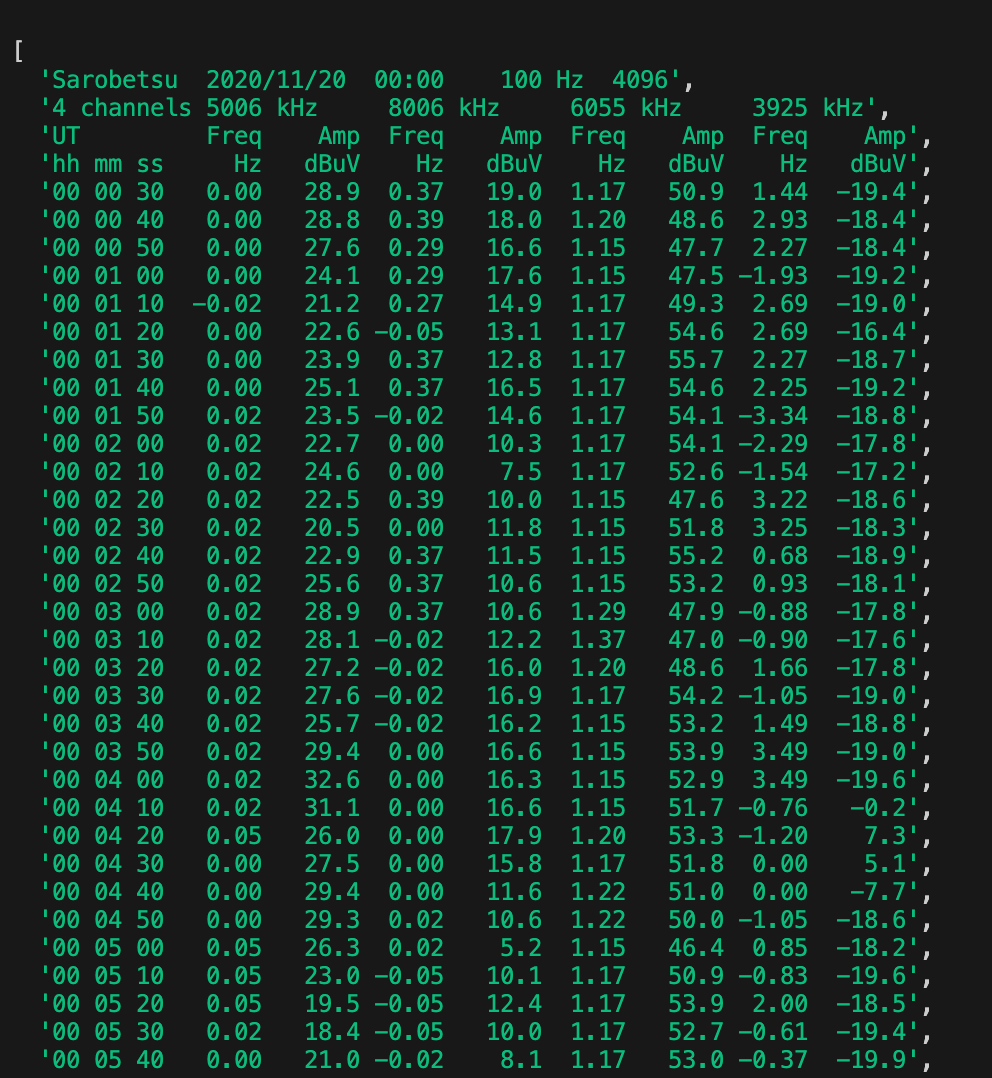
\includegraphics[width=70mm]{fig/textdata.png}
 \end{figure}
%%%%%%%%%%%%%%%%%%%%%%%%%%%%%%%%%%%%%%%%%%%%%%%%%%%%%%
\subsection{完成品}
 完成したサイトがこちらになります.
%%%%%%%%%%%%%%%%%%%%%%%%%%%%%%%%%%%%%%%%%%%%%%%%%%%%%%
\small
\begin{thebibliography}{99}
\setlength{\itemsep}{0pt}
\smallskip

\bibitem{hfd_report}
吉川晃平,HFドップラーにより観測された地震に伴う電離圏変動の中性待機波導数値シミュレーションによる定量的評価,電気学会論文誌A Vol.136 No.5 pp.259~264

\bibitem{next}
Next.js by Vercel - The React Framework
\url{https://nextjs.org/} 2024/1/13

\bibitem{shu_sotsuken}
中嶋柊,HF ドップラー観測データの利活用を目的とする web アプリケーションのフロントエンド設計,令和4年度 制御情報システム創造演習 報告書

\bibitem{superagent}
Superagent-npm 
\url{https://www.npmjs.com/package/superagent}  2023/01/25

\bibitem{cheerio}
cheeriojs/cheerio: Fast, flexible, and lean implementation of core jQuery designed specifically for the server. 
\url{https://github.com/cheeriojs/cheerio}  2023/01/25 

\bibitem{hfd_link}
HF Doppler Sounding Experiment in Japan - HFDOPE
\url{http://gwave.cei.uec.ac.jp/~hfd/pre.html} 2024/13

\end{thebibliography}
\normalsize
%%%%%%%%%%%%%%%%%%%%%%%%%%%%%%%%%%%%%%%%%%%%%%%%%%%%%%





